\chapter{Vorbereitung}

\section{Der klassische Hall-Effekt}

Der klassische Hall-Effekt beschreibt den Effekt eines Magnetfeldes auf eine
Probe. So baut sich im Inneren der Probe ein elektrisches Feld auf, dessen
resultierende elektrische Kraft im stationären Zustand gerade die Lorentz-Kraft
kompensiert.\\
Zur Diskussion beginnt man mit der klassischen Bewegungsgleichung im Magnetfeld:
\[
    m^* \dot{\vec{v}} = - e \left( \vec{E} + \vec{v}_d \times \vec{B} \right)
                      - m^* \frac{\vec{v}_d}{\tau}
\]
Hierbei bezeichnet $\vec{v}_d$ die Driftgeschwindigkeit, $\tau$ die mittlere
Stoßzeit, $m^*$ die effektive Masse, $\vec{E}$ das elektrische Feld und $\vec{B}$
das Magnetfeld. Der Term $-e \vec{E}$ beschreibt die durch das elektrische 
Gleichfeld auf die Elektronen wirkende konstante Kraft. Der letzte Teil 
$m \, \vec{v_d} / \tau$ berücksichtigt die hemmende Wirkung der Stöße. 
Da die Elektronen bei jedem Stoß ihre Bewegungsrichtung ändern, bleibt außerdem
nur der durch die Driftgeschwindigkeit verursachte Beitrag 
$-e \left( \vec{v}_d \times \vec{B} \right)$ übrig.\\
Zur Vereinfachung betrachten wir ein in $z$-Richtung anliegendes Magnetfeld
im stationären Fall, also $\dot{\vec{v}} = 0$. Somit ergibt sich:
\begin{align*}
    \vec{v}_{d,x} &= - \frac{e \tau}{m^*} \left( E_x + \vec{v}_{d,y} \; B \right),\\
    \vec{v}_{d,y} &= - \frac{e \tau}{m^*} \left( E_y + \vec{v}_{d,x} \; B \right),\\
    \vec{v}_{d,x} &= - \frac{e \tau}{m^*} E_z
\end{align*}
Mit der Beweglichkeit $\mu = e \tau / m$ und der Elektronendichte
\[
    j = -e n \vec{v}_d = \frac{n e^2 \tau}{m} \vec{E} = n e \mu E
\]
aus der für die elektrische Leitfähigkeit folgt
\[
    \sigma = \frac{j}{E} = \frac{n e^2 \tau}{m} = n e \mu
\]
folgt für die Stromdichte im betrachteten Fall:
\[
    \begin{pmatrix}
        j_x\\ j_y \\ j_z
    \end{pmatrix} 
    = - \frac{\sigma_0}{1 + \omega_c^2 \tau^2}
      \begin{pmatrix}
          1             & -\omega_c \tau    & 0 \\
          \omega_c \tau & 1                 & 0 \\
          0             & 0                 & 1+\omega_c^2 \tau^2 \\
      \end{pmatrix}
      \begin{pmatrix}
          E_x \\ E_y \\ E_z
      \end{pmatrix}
\]
Hier bezeichnet $\omega_0 = n e^2 \tau / m^*$ die Leitfähigkeit ohne Magnetfeld
und $\omega_c$ für die Zyklotronfrequenz.\\
Zur Vereinfachung betrachten wir einen flachen Stab mit rechteckigen Querschnitt.
Der Strom fließt hierbei in $x$-Richtung. Mit dieser Geometrie tritt in
$z$-Richtung kein elektrisches Feld auf. Somit vereinfacht sich obiger Ausdruck zu:
\[
    \begin{pmatrix}
        j_x \\ j_y
    \end{pmatrix}
    = \begin{pmatrix}
         \omega_{xx} & \omega_{xy} \\
        -\omega_{xy} & \omega_{xx}
      \end{pmatrix}
      \begin{pmatrix}
          E_x \\ E_y
      \end{pmatrix}
\]
Hier wurden die Leitwerte
\[
    \omega_{xx} = \frac{ne}{B} \frac{\omega_c \tau}{1+\omega_c^2 \tau^2}, \qquad
    \omega_{xy} = -\frac{ne}{B} \frac{\omega_c^2 \tau^2}{1+\omega_c^2 \tau^2}
\]
eingeführt.\\
Löst man das Gleichungssystem nach den elektrischen Feldern auf erhält man:
\[
    \begin{pmatrix} E_x \\ E_y \end{pmatrix}
    = \begin{pmatrix}
         \rho_{xx} & \rho_{xy} \\
        -\rho_{xy} & \rho_{xx} 
      \end{pmatrix}
      \begin{pmatrix}
          j_x \\ j_y
      \end{pmatrix}
\]
mit den spezifischen Widerständen:
\[
    \rho_{xx} = \frac{B}{ne} \frac{1}{\omega_c \tau} = \frac{m^*}{ne^2\tau}, \qquad
    \rho_{xy} = \frac{B}{ne}
\]
Hier wird $\rho_{xx}$ als Längswiderstand $R$ und $\rho_{xy}$ als Hall-Widerstand
$R_H$ bezeichnet.
In einem anisotropen Medium würden die Größen $\rho_{yx}$ und $\rho_{yy}$
auftreten. Für isotrope Medien, die hier betrachtet werden sollen, gilt jedoch:
$\rho_{xx} = \rho_{yy}$ und $\rho_{yx} = - \rho_{xy}$. Ein Plot der klassischen
Widerstände ist in Abbildung \ref{Abb:klassisch} zu sehen.
\begin{figure}
    \centering
        \begin{subfigure}[c]{0.45\textwidth}
        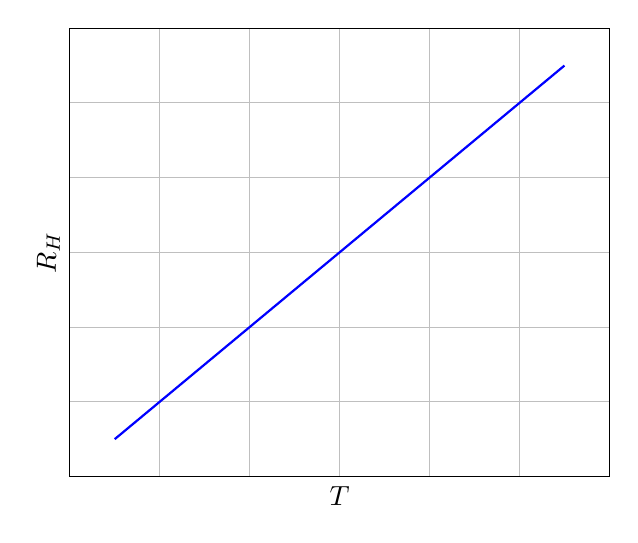
\begin{tikzpicture}
            \begin{axis}[
                ticks=none,
                xlabel={$T$}, ylabel={$R_H$},
                grid=both
            ]
                \addplot[thick, blue] {x};
            \end{axis}
        \end{tikzpicture}
        \caption{Hall-Widerstand}
    \end{subfigure}
    \begin{subfigure}[c]{0.45\textwidth}
        \begin{tikzpicture}
            \begin{axis}[
                ticks=none,
                xlabel={$T$}, ylabel={$R_\square$},
                grid=both
            ]
                \addplot[thick, blue] {1};
            \end{axis}
        \end{tikzpicture}
        \caption{Schichtwiderstand}
    \end{subfigure}

    \caption{Widerstände beim klassischen Hall-Effekt}
    \label{Abb:klassisch}
\end{figure}

\begin{figure}
    \centering
    \def\svgwidth{0.6\linewidth}
    \import{Abb/}{Abb/quanten_hall.pdf_tex}
    \caption{Hall und Schichtwiderstand beim Quanten-Hall-Effekt}
    \label{vorb:qh}
\end{figure}
